\chapter{Projektorganisation}
\section{Vorgehen}
Das Projekt wurde in den Grunds�tzen an den RUP\footnote[1]{Rational Unified Process: \href{https://de.wikipedia.org/wiki/Rational\_Unified\_Process}{https://de.wikipedia.org/wiki/Rational\_Unified\_Process}} Prozess angelegt. Als wichtigstes Merkmal wurden die Projektphasen Inception, Elaboration, Construction 1, Construction 2, Construction 3 und Transition definiert.
\section{Risiken}
\section{Meilensteine}
Die Meilensteine wurden ebenfalls an den RUP Prozess angelegt und sind so meist bei den �berg�ngen in die n�chste Phase definiert. In der nachfolgenden Tabelle sind die definierten Meilensteine des Projektes nach Datum geordnet:

\begin{center}

	\bgroup
	\def\arraystretch{1.5}
    \begin{tabular}{ | c | l | p{13cm} |} \hline
    
    \textbf{Nr.} & \textbf{Datum} & \textbf{Beschreibung} \\ \hline
    
    001 & 23.10.2016 & \textbf{Einlesen und Spektrometer�bergabe} \newline
    Die Spektrometer konnten von den Studierenden in Empfang genommen werden. \\ \hline
    
    002 & 30.11.2016 & \textbf{Anforderungen} \newline
    Das Pflichtenheft wurde erstellt und vom Kunden akzeptiert. \\ \hline
    
    003 & 30.11.2016 & \textbf{Proof of Concept} \newline
    Es liegt ein funktionierender Proof of Concept vor der die Verbindung zum Spektrometer herstellen und Antworten empfangen kann. \\ \hline
    
    004 & 21.12.2016 & \textbf{Prototyp 1} \newline
    Ein funktionierender Prototyp mit allen Anforderungen der Priorit�t 1 ist f�r den Kunden im TestFlight freigegeben. \\ \hline
    
    005 & 25.01.2017 & \textbf{Prototyp 2} \newline
    Ein funktionierender Prototyp mit allen Anforderungen der Priorit�t 2 ist f�r den Kunden im TestFlight freigegeben. \\ \hline
    
    006 & 01.03.2017 & \textbf{Version 1.0} \newline
    Eine funktionierende Version der App mit allen Anforderungen der Priorit�t 3 ist f�r den Kunden im TestFlight freigegeben. \\ \hline
    
    007 & 16.03.2017 & \textbf{Projektabschluss} \newline
    Die finale Version mit allen Fehlerverbesserungen aus Version 1.0 ist im TestFlight f�r den Kunden freigegeben. \\ \hline
    
    \end{tabular}
    \egroup
    
\end{center}

\section{Zeitplanung}
Die Zeitplanung wurde mithilfe der RUP Phasen durchgef�hrt. Damit konnte die Dauer der einzelnen Phasen abgesch�tzt und mit den Meilensteinen abgestimmt werden. Es musste noch auf einige Abwesenheiten des Kunden geachtet werden und somit die Meetings f�r die Prototyp Pr�sentation etwas vor- oder nach den jeweiligen Releasedaten der Prototypen angesetzt werden. Der Zeitplan befindet sich in detaillierter Form auch im Anhang.

\begin{figure}[h]
	\begin{center}
		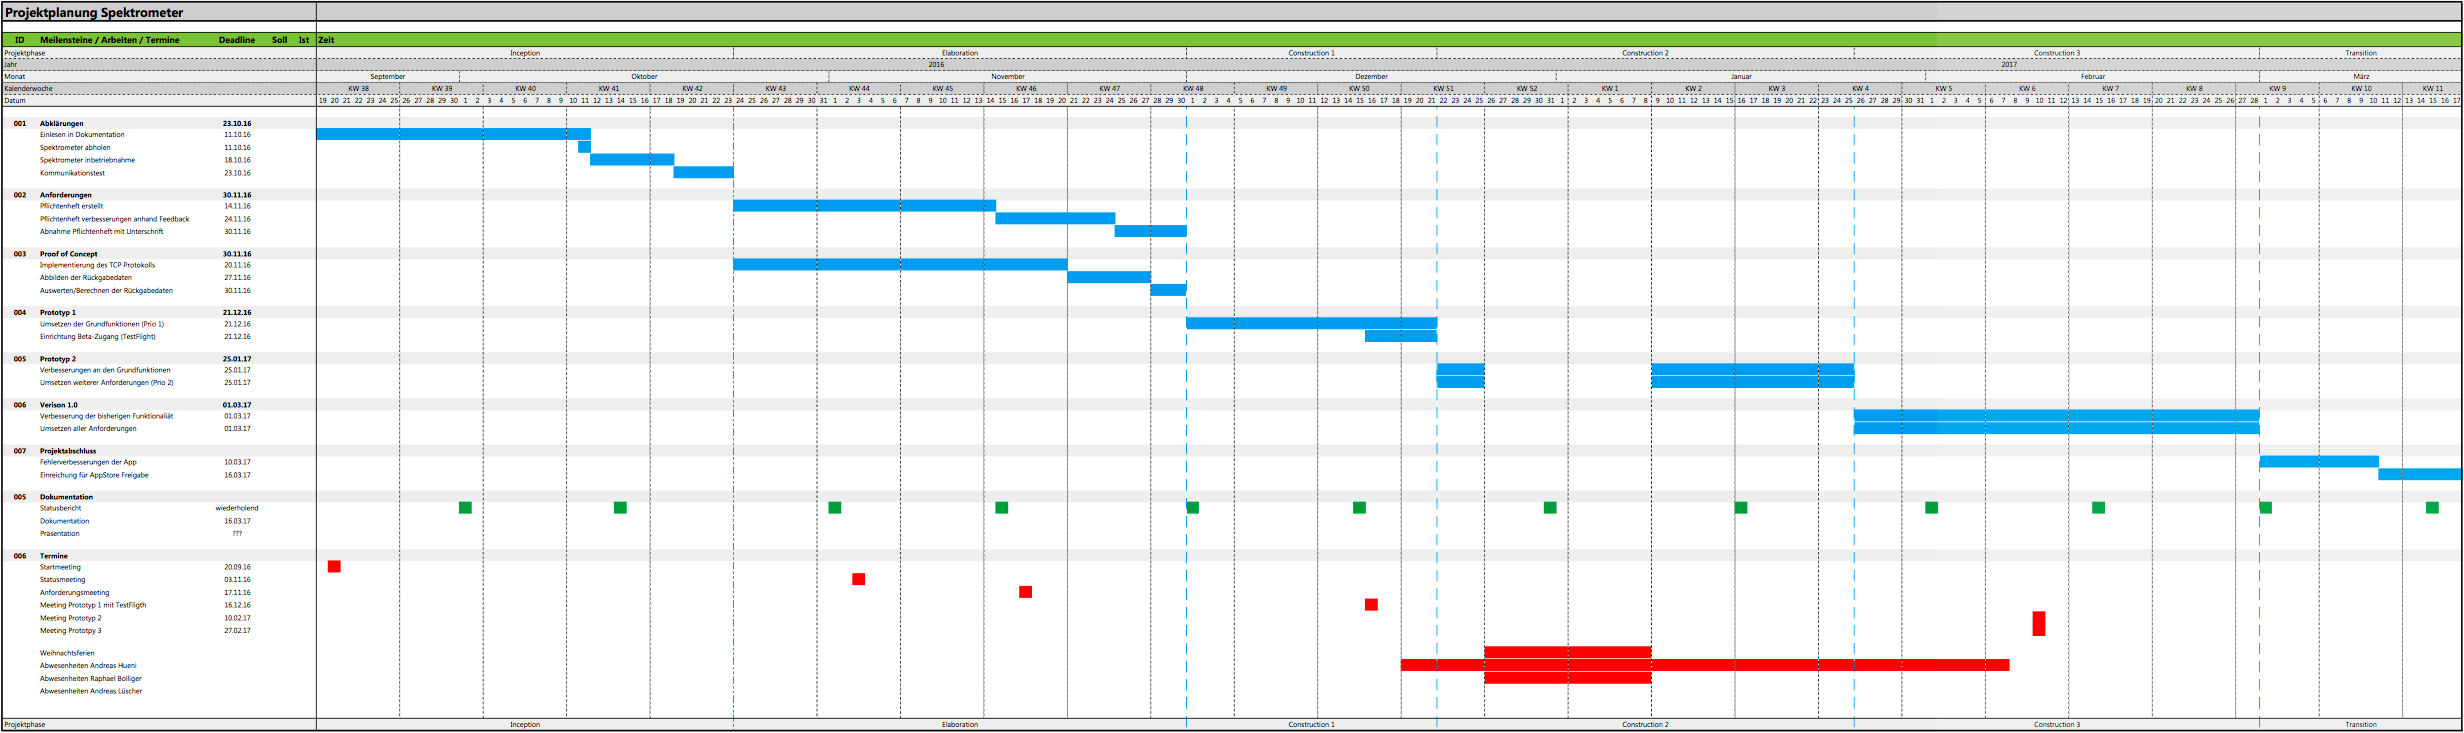
\includegraphics[scale=0.19]{images/TimePlanning} 
	\caption{Zeitplanung}
	\label{fig:TimePlanning}
	\end{center}
\end{figure}

\section{Anforderungen}
Die Anforderungen wurden zu beginn bei einem Startmeeting mit dem Kunden besprochen. Weiter konnten viele Anforderungen detailliert in der bestehenden Software ausgemacht werden. 

\section{Arbeitspakete}

\section{Soll- und Istvergleich}